%
% Copyright 2018 Markus Borg, Lund University
%
% This work is licensed under a Creative Commons Attribution-ShareAlike 4.0 International License.
% See http://creativecommons.org/licenses/by-sa/4.0/
%
% The dodument is based on a LaTeX template developed by Jean-Philippe Eisenbarth
% https://github.com/jpeisenbarth/SRS-Tex
%
\documentclass{scrreprt}
\usepackage{graphicx}
\usepackage{listings}
\usepackage{underscore}
\usepackage[bookmarks=true]{hyperref}
\usepackage[utf8]{inputenc}
\usepackage[english]{babel}
\hypersetup{
    bookmarks=false,    % show bookmarks bar?
    pdftitle={Lab 3},    % title
    pdfauthor={Markus Borg},                     % author
    pdfsubject={TeX and LaTeX},                        % subject of the document
    pdfkeywords={TeX, LaTeX, graphics, images}, % list of keywords
    colorlinks=true,        % false: boxed links; true: colored links
    linkcolor=blue,         % color of internal links
    citecolor=black,        % color of links to bibliography
    filecolor=black,        % color of file links
    urlcolor=purple,        % color of external links
    linktoc=page            % only page is linked
}%
\def\myversion{1.4 }
\date{}
%\title
\usepackage{hyperref}
\begin{document}

\begin{flushright}
    \rule{16cm}{5pt}\vskip1cm
    \begin{bfseries}
    	\LARGE{ETSA02-ADM-LAB3}\\
    	\vspace{1.5cm}
        \Huge{Lab 3}\\
        \vspace{0.5cm}
        Automated system testing\\
        \vspace{0.5cm}
        with RobotTestBed\\
        \vspace{1.5cm}
        \LARGE{Version \myversion approved}\\
        \vspace{1.5cm}
        Prepared by Markus Borg\\
        %\vspace{1.5cm}
        Dept. of Computer Science, Lund University\\
        \vspace{1.5cm}
        \today\\
    \end{bfseries}
\end{flushright}

%\tableofcontents

\chapter*{Revision History}

\begin{center}
    \begin{tabular}{|c|c|c|c|}
        \hline
	    Name & Date & Reason For Changes & Version\\
        \hline
	    Markus Borg & 2018-03-21 & Initial draft. & 0.1\\
        \hline
        Markus Borg & 2018-04-01 & First instructions for the RobotTestBed. & 0.2\\
        \hline
        Markus Borg & 2018-04-04 & Drafted introduction section. & 0.3\\
        \hline
        Markus Borg & 2018-04-07 & Complete draft, ready for internal review. & 0.4\\
        \hline
        Markus Borg & 2018-04-16 & Updated after internal review. & 0.5\\
        \hline
        Markus Borg & 2018-04-17 & Ready for lab. & 1.0\\
        \hline
        Markus Borg & 2019-04-07 & Updated for introsofteng-botexample. Simplified. & 1.1\\
        \hline
        Markus Borg & 2019-04-09 & Corrected the string to the robot under test. & 1.2\\
        \hline
        Markus Borg & 2019-04-16 & Clarified that teams are not supported by RobotTestBed. & 1.3\\
        \hline
        Markus Borg & 2019-05-03 & Relaxed some requirements to simplify testing. & 1.4\\
        \hline
    \end{tabular}
\end{center}

\chapter{Introduction}
During Lab 3 you will continue working with automated testing of Basic Melee Bot. You will still use the JUnit framework to drive the test automation, but your test design will leave the unit level to instead target robot behavior on the system level. To enable such testing, you will work with the Robocode plug-in RobotTestBed. Furthermore, you will design test cases to verify quality requirements regarding the battle performance of Basic Melee Bot. More specifically, Lab 3 covers:

\begin{itemize}
\item Working with the RobotTestBed plugin.
\item Designing JUnit test cases for system testing.
\item Designing JUnit test cases for testing quality requirements.
\end{itemize}

\vspace{1em}
\fbox{\begin{minipage}{0.99\textwidth}
\textbf{Note!} Robot teams are not supported by RobotTestBed. Any attempt to field a team of robots directly from a system test case will fail. If you have specified corresponding quality requirements for your robot under development, you will have to design \textit{manual} test cases to verify them, i.e., start a new battle in Robocode and verify that the intended behavior can be observed.
\end{minipage}}
\vspace{1em}

\chapter{Before the lab}
You shall continue working on the source code you developed for Lab~2. If you have not yet completed the code to make ``wall avoidance'' work for the Lab~2 robot, please do so now. Before continuing with Lab~3, start Robocode and verify that Basic Melee Bot does not get stuck in any walls. The content in the Package Explorer should resemble Figure~\ref{fig:packageExplorer}.

\begin{figure}
\centering
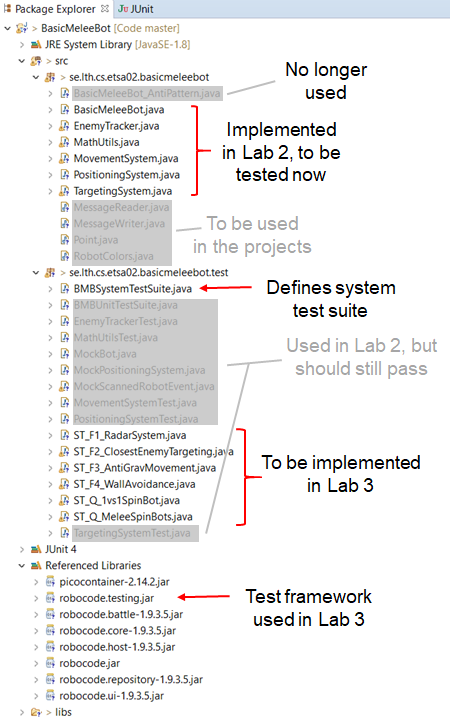
\includegraphics[width=0.75\textwidth]{figures/packageExplorerAfterLab2.png}
\caption{The Package Explorer in Eclipse after completing Lab 2. In Lab 3 you will implement the system test cases with the prefix `ST'. `F1-F4' refers to the four features of Basic Melee Bot, and `Q' indicates that a quality requirement is under test. You will now work with the unit test suite in Lab 3, but all unit test cases should of course still pass.}
\label{fig:packageExplorer}
\end{figure}

\section{Install, setup, and run test cases with RobotTestBed and JUnit}
Follow the instructions below to install the Robocode testing plugin and setup JUnit for system testing of robots. Figure~\ref{fig:overview} shows an overview of the setup we will use in Lab~3.

\begin{figure}
\centering
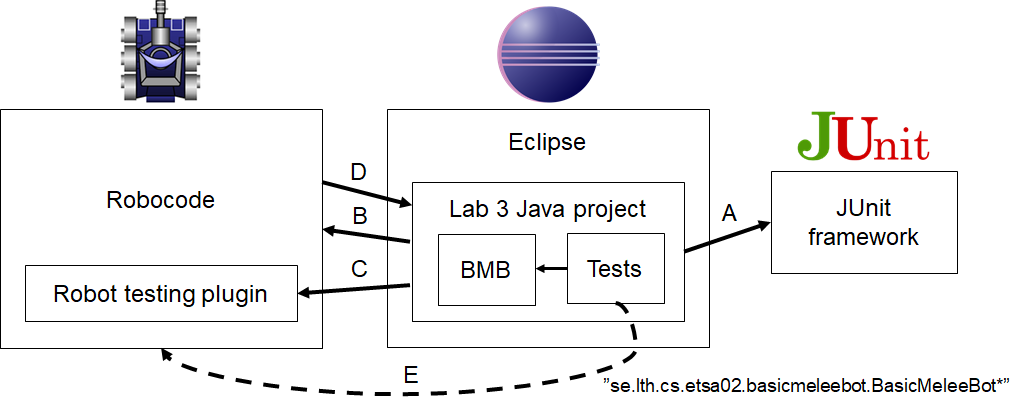
\includegraphics[width=0.85\textwidth]{figures/overview.png}
\caption{The three main elements in the Lab 3 setup, and the key links A-E. To the left, your local Robocode installation with the new Robot testing plugin. The link from Robocode to the Lab 3 Java project (cf. D) is configured in the Robocode options menu. In the middle, your Java project containing BasicMeleeBot (BMB) and its test cases. The references to Robocode (cf. B) and to Robot testing plugin (cf. C) are configured in the ``Java build path'' in Eclipse. To the right, the JUnit framework. The Java project in Eclipse needs a reference to the JUnit library (cf. A). Finally, the test cases contain a string to explicitly specify which Robocode robot is under test (cf. E) -- this should for all test cases be ``se.lth.cs.etsa02.basicmeleebot.BasicMeleeBot*'' (unless you have renamed your project or robot).}
\label{fig:overview}
\end{figure}

\begin{enumerate}
\item \textbf{Download Robot testing plugin}. Download the latest Robot testing plugin (1.9.3.7) from https://sourceforge.net/projects/robocode/files/robocode/1.9.3.7/ -- The file is called ``robocode.testing-1.9.3.7-setup.jar''
\item \textbf{Install Robot testing plugin}. Run\footnote{In a terminal (or command prompt) type java -jar robocode.testing-1.9.3.7-setup.jar} the downloaded jar file and 
install the Robot testing plugin. The default option is to install the plugin in the existing Robocode folder -- this is correct.
\item \textbf{Create a JUnit run configuration}. In Eclipse, right click ``BMBSystemTestSuite.java'' and choose ``Run as..'' and create a new JUnit run configuration. Give the configuration a descriptive name, such as ``Lab3 system tests''. Do this in the same way as when creating a normal JUnit run configuration (i.e., Lab 2), but you must also add -Drobocode.home=PATH\_TO\_ROBOCODE as an argument to the VM (in the second tab, in the second text field).\\\\Note: You must replace PATH\_TO\_ROBOCODE with the installation path of Robocode on your computer. Please refer to Figure~\ref{fig:runConfig} for an example.
\end{enumerate}

\begin{figure}
\centering
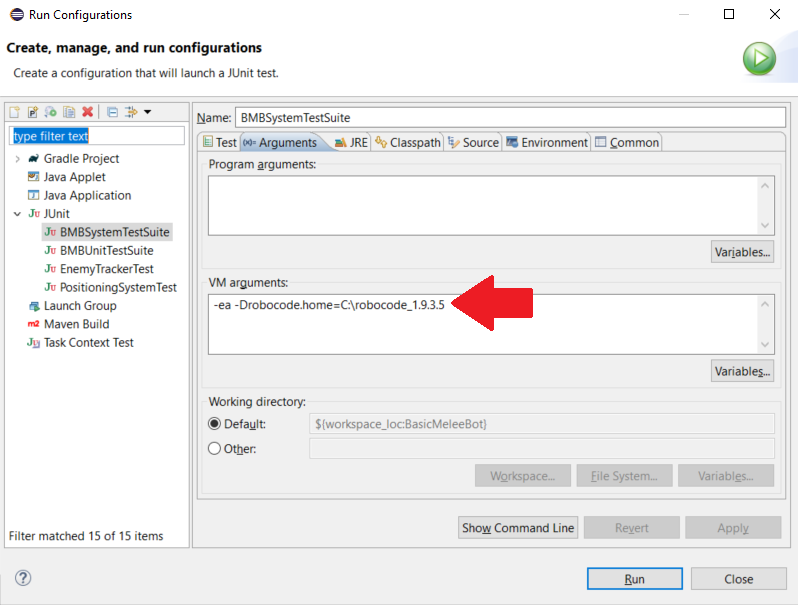
\includegraphics[width=0.85\textwidth]{figures/runConfig.png}
\caption{Example of arguments for a JUnit run configuration corresponding to Robocode being installed in ``C:\textbackslash robocode\_1.9.3.5''. Note: you should install 1.9.3.7.}
\label{fig:runConfig}
\end{figure}

\vspace{1em}
\fbox{\begin{minipage}{0.99\textwidth}
\textbf{Note!} Previous students have reported that there is a bug in RobotTestBed that manifests in some operational environments. If RobotTestBed cannot find your robots, i.e., if you get a NullPointerException from the RepositoryManager in Robocode, try adding \texttt{-DNOSECURITY=true} as a parameter to the VM.
\end{minipage}}
\vspace{1em}

\newpage

\section{The fundamentals of RobotTestBed}
To get an initial understanding of RobotTestBed, study the simple example TestWallBehavior that follows. The test case verifies that the corresponding robot visits all four corners of the battlefield. RobotTestBed lets you override methods in Robocode's BattleAdaptor to add JUnit assertions for testing robot behavior. The complete list is available in the Robocode API, but a handful of methods should be enough for Lab 3:
\begin{itemize}
\item public void onBattleCompleted(BattleCompletedEvent event)
\item public void onRoundStarted(RoundStartedEvent event)
\item public void onRoundEnded(RoundEndedEvent event)
\item public void onTurnEnded(TurnEndedEvent event)
\end{itemize}

During the lab, you will work on designing test cases to verify the three primary features of Basic Melee Bot: 1) Spinning radar, 2) Closest enemy targeting,  and 3) Wall avoidance. You will also design a test case to verify a quality requirement related to 1-vs-1 battle performance. To support this, you will get examples of how you could test the feature ``Non-stop anti-gravity movement'' and the quality requirement related to Melee battle performance. You can study the features and requirements of Basic Melee Bot in Section~\ref{sec:atlab}. 

\newpage
\begin{verbatim}
/**
 * Copyright (c) 2001-2018 Mathew A. Nelson and Robocode contributors
 * All rights reserved. This program and the accompanying materials
 * are made available under the terms of the Eclipse Public License v1.0
 * which accompanies this distribution, and is available at
 * http://robocode.sourceforge.net/license/epl-v10.html
 */
package sample;

import static org.junit.Assert.assertTrue;
import robocode.control.events.BattleCompletedEvent;
import robocode.control.events.TurnEndedEvent;
import robocode.control.snapshot.IRobotSnapshot;
import robocode.control.testing.RobotTestBed;

/**
 * Tests that sample.Walls moves to all four corners.
 *
 * @author Philip Johnson (original)
 * @author Pavel Savara (contributor)
 */
public class TestWallBehavior extends RobotTestBed {

	/**
	 * True if the robot visited this corner during the test case.
	 */
	boolean visitedUpperLeft = false;

	/**
	 * True if the robot visited this corner during the test case.
	 */
	boolean visitedUpperRight = false;

	/**
	 * True if the robot visited this corner during the test case.
	 */
	boolean visitedLowerLeft = false;

	/**
	 * True if the robot visited this corner during the test case.
	 */
	boolean visitedLowerRight = false;

	/**
	 * Specifies that SittingDuck and DaCruzer are to be matched up in this test case.
	 *
	 * @return The comma-delimited list of robots in this match.
	 */
	@Override
	public String getRobotNames() {
      return "sample.SittingDuck,sample.Walls";
	}

	/**
	 * This test runs for 1 round.
	 *
	 * @return The number of rounds.
	 */
	@Override
	public int getNumRounds() {
      return 1;
	}

	/**
	 * After each turn, check to see if we're at a corner.
	 * If so, set the corresponding flag.
	 *
	 * @param event Info about the current state of the battle.
	 */
	@Override
	public void onTurnEnded(TurnEndedEvent event) {
      IRobotSnapshot robot = event.getTurnSnapshot().getRobots()[1];
      double xPos = robot.getX();
      double yPos = robot.getY();

      if ((xPos < 40) && (yPos < 40)) {
        visitedUpperLeft = true;
      }
      if ((xPos < 40 && (yPos > (height - 40)))) {
        visitedLowerLeft = true;
      }
      if ((xPos > (width - 40)) && (yPos < 40)) {
        visitedUpperRight = true;
      }
      if ((xPos > (width - 40) && (yPos > (height - 40)))) {
        visitedLowerRight = true;
      }
	}

	/**
	 * After the battle, check to see that we've visited the corners.
	 *
	 * @param event Details about the completed battle.
	 */
	@Override
	public void onBattleCompleted(BattleCompletedEvent
			event) {
      assertTrue("Check UpperLeft", visitedUpperLeft);
      assertTrue("Check LowerLeft", visitedLowerLeft);
      assertTrue("Check UpperRight", visitedUpperRight);
      assertTrue("Check LowerRight", visitedLowerRight);
  }
}
\end{verbatim}

\chapter{At the lab} \label{sec:atlab}
In Lab 3, your task is to design automated test cases that verify features and detailed requirements of Basic Melee Bot. This is far from trivial, as all robot states are not observable when working with RobotTestBed. A considerable challenge in Lab 3, and in the project in general, is to create as good test cases as possible given the constraints imposed by RobotTestBed. For some requirements, you might have  to argue that you will have to rely on code reviews for verification. However, in most cases you should be able to design test cases that -- at least partly -- verify the requirements in question. Software testing is a creative activity, and sometimes more demanding than implementing the actual features in source code.

Below you will find the four features of Basic Melee Bot and two quality requirements, listed in the recommended implementation order. All items listed below have a corresponding test case in the test src/test folder. Implement the test cases in the prepared files (ST_FX or ST_Q prefixes) and make sure they all pass in JUnit. We suggest that you complete Lab 3 in the following order:

\begin{enumerate}
\item Study how Feature 3 ``Non-stop anti-gravity movement'' is tested in\\ \texttt{ST_F3_AntiGravMovement.java}.
\item Implement a test case for Feature 4: ``Wall avoidance'' in\\ \texttt{ST_F4_WallAvoidance.java}.
\item Study how the Quality requirement ``Melee battle performance'' is tested in\\ \texttt{ST_Q_MeleeSpinBots.java}.
\item Implement a test case for the Quality requirement ``1-vs-1 battle performance'' in \texttt{ST_Q_1vs1SpinBot.java}.
\item Implement a test case for Feature 2: ``Closest enemy targeting'' in\\ \texttt{ST_F2_ClosestEnemyTargeting.java}.
\item (Optional) Try to implement a test case for ``Feature 1: Spinning radar'' in\\ \texttt{ST_F1_RadarSystem.java}.
\end{enumerate}

\section{Feature 3 -- Non-stop anti-gravity movement}
BMB shall use anti-gravity movement.
	
\subsection{Description and Priority}
Anti-gravity movement is used to keep a distance to certain points on the battlefield. BMB shall use this movement to stay away from enemy robots. Furthermore, to avoid becoming an easy target, BMB shall never stay still in one position for too long.\\\\Business priority: \textbf{medium}\\
Implementation risk: \textbf{medium}

\subsection{Functional Requirements}
\begin{itemize}
\item[REQ-F3-1] BMB shall continuously move away from enemy robots.
\item[REQ-F3-2] BMB shall never stay in the same position for more than 40 consecutive turns.
\end{itemize}

\section{Feature 4 -- Wall avoidance}
BMB shall avoid driving into walls.

\subsection{Description and Priority}
Crashing into walls damages robots and forces them into a stop. BMB shall not end up in walls, even when the anti-gravity movement suggests such positions.\\\\Business priority: \textbf{medium}\\
Implementation risk: \textbf{medium}

\subsection{Functional Requirements}
\begin{itemize}
\item[REQ-F4-1] When closer than 15 distance units to a wall, BMB shall alter its course to avoid collision.
\end{itemize}

\section{Quality Requirements}
This section describes quality requirements for Basic Melee Bot. The robot is primarily intended for use in the LU Rumble, but it shall also be competitive in 1-vs-1 battles and melee battles.

\subsection{1-vs-1 Battle Performance Requirements}
When Basic Melee Bot battles against a single enemy robot, it will continuously change its position on the battlefield and stay away from the enemy robot by using its non-stop anti-gravity movement. Basic Melee Bot shall perform well against the Robocode sample robots.

\begin{itemize}
\item[REQ-Q1] Basic Melee Bot shall have at least 51\% win rate against SpinBot in battles over 100 rounds on a 800x600 battlefield (standard Robocode size for 1-vs-1 battles).
\end{itemize}

\subsection{Melee Battle Performance Requirements}
When Basic Melee Bot battles against multiple enemy robot, it will try to stay away from enemy robots by using its non-stop anti-gravity movement. Basic Melee Bot shall perform well in melee battles against the Robocode sample robots.

\begin{itemize}
\item[REQ-Q2] Basic Melee Bot shall have at least 26\% win rate in melee battles against three enemy SpinBots in battles over 100 rounds on a 1000x1000 battlefield (standard Robocode size for melee battles).
\end{itemize}

\vspace{1em}
\fbox{\begin{minipage}{0.99\textwidth}
\textbf{Note!} Minor differences in the implementation of Basic Melee Bot might result in considerably weaker battle performance. If your related test cases do not pass, try relaxing the win rates until they pass. Discuss the situation with your lab assistant.
\end{minipage}}
\vspace{1em}

\section{Feature 2 -- Closest enemy targeting}
BMB shall target and shoot at the closest enemy robot.

\subsection{Description and Priority}
The rationale behind targeting and shooting at the closest enemy is that nearby robots are easier to hit. The solution is simple but useful.\\\\Business priority: \textbf{high}\\
Implementation risk: \textbf{low}

\subsection{Functional Requirements}
\begin{itemize}
\item[REQ-F2-1] BMB shall fire at the closest enemy robot as long as the battle is ongoing.
\item[REQ-F2-2] BMB shall use a constant fire power of 1.
\end{itemize}

\begin{center}
\textbf{------ REACH THIS POINT TO PASS LAB 3! ------}
\end{center}

\section{Feature 1 -- Spinning radar}
BMB shall feature a spinning radar.

\subsection{Description and Priority}
The spinning radar is a simple solution to detect enemy robots by continuously scanning the entire battlefield.\\\\Business priority: \textbf{high}\\
Implementation risk: \textbf{very low}

\subsection{Functional Requirements}
\begin{itemize}
\item[REQ-F1-1] The radar shall scan the battlefield clockwise as long as BMB is operational and the battle is ongoing.
\item[REQ-F1-2] Detected enemy robots shall be stored in an internal data structure. 
\end{itemize}

\chapter{After the lab}
In the project, your group should verify all requirements specified in your Software Requirements Specification. Reflect on the testability of robots developed in Robocode. What is particularly difficult to test with RobotTestBed? Can you specify requirements in a way that supports software testing? Your group might end up in a trade-off between specifying something amazing that cannot be dynamically  tested versus specifying something less amazing that can be tested exhaustively. What will you prioritize? And how will you build your arguments around requirements that have been only statically tested, or only partly tested using unit testing?

\end{document}
